\section{Implementation}\label{sec:03_impl}
% Explain section
This section explains the implementation based on the conceptual design introduced in \Sec{sec:02_design}. 
% MVC
As mentioned in PROBLM, the MVC architecture is used to implement this application.
% What is what
The models are introduced in \Sec{subsec:03_impl_models}, the views and controllers in \Sec{subsec:03_impl_servlets}.
% Others
Additionally, this implementation uses custom object stores (introduced in \Sec{subsec:03_impl_objstores}) and filters (introduced in \Sec{subsec:03_impl_filters}).


% !!!!
% MVC
% JAVA BEANS
% ...

% Object Store (User, Rooms, all Models + Beans)


\subsection{Models}\label{subsec:03_impl_models}
% Intro
As being mentioned, this project is implemented using the MVC pattern. Therefore, each entity of the chat system is represented by a model.
% Beans
Each model is implemented using the Java Bean specification. This enables to reuse models in \texttt{JSP} files.

% Figure
\begin{figure}[h]
\centering
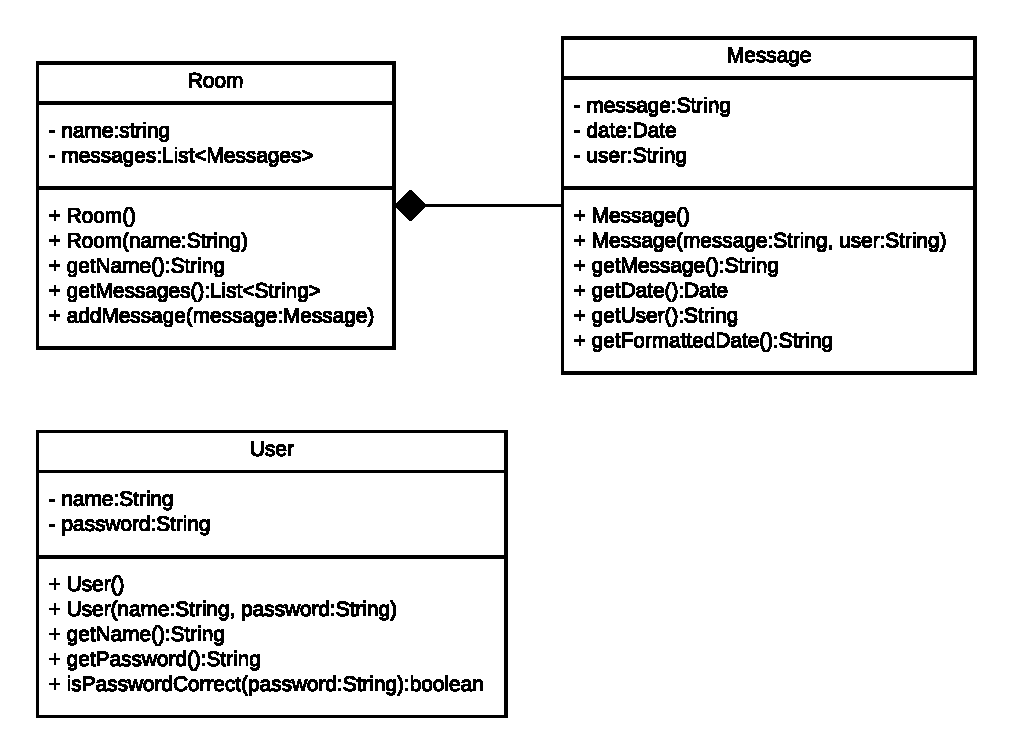
\includegraphics[scale=0.8]{images/03_impl/models}
\caption{Used models for the chat system}
\label{fig:03_impl_models_models}
\end{figure}

% Explain Figure
\Fig{fig:03_impl_models_models} shows all models used in the implementation of the chat system.
% Room and message
A \texttt{Room} models exists, which represents a room where users can chat with each other. Therefore, multiple messages are saved in a \texttt{Room}. A \texttt{Message} model represents a message send by any user in a specific room. Each \texttt{Message} is identified by its message-text, the name of the user, and the date when it was send.
% User
Each user is represented by a \texttt{User} model. This model is identified by the username, and the password.


% ==============
% ==============
\subsection{Object Stores}\label{subsec:03_impl_objstores}
% Why
As being mentioned in SEC DESIGN STORAGE, a custom store is needed to save the in \Sec{subsec:03_impl_models} introduced models.

Therefore, the following stores are being implemented:
\begin{itemize}
\item \texttt{UserStore}, saves \texttt{User} models
\item \texttt{RoomStore}, saves \texttt{Room} models
\end{itemize}
% Store functionality
Because a user and room can only exists once, a \texttt{Set}\footnote{Set (Java Platform SE 8) - \url{https://docs.oracle.com/javase/8/docs/api/java/util/Set.html}} data structure is used to save both Users, and Rooms. Furthermore, a store needs to provide the functionality to add an object to the store, get all objects from the store, or a specific one, and to check if an object has already been added to the store.


% Abstract class
Therefore, an abstract class called \texttt{ObjectsStore} is implemented, which implements the previously mentioned functionalities.
% Generics
The \texttt{ObjectStore} uses generics to implement the properties and methods. The \texttt{UserStore} and \texttt{RoomStore} implement this \texttt{ObjectStore} class and set the model (\texttt{User} and \texttt{Room}, respectively) for the generic type.
% Lifetime
The lifetime of an object saved to a store, is equal to the lifetime of the running webserver. As long as the webserver is running, an the objects are saved to memory.
% Lifetime of user
Except for the \texttt{UserStore}, which reads all \texttt{User} models from a text file, and write Users to a text file. Therefore, when the server restarts, all previously added \texttt{User} modes are available again.

%
% SINGLETON PATTERN !!!
%


% ==============
% ==============
\subsection{Servlets}\label{subsec:03_impl_servlets}
Fig XY shows the architecture of the in SEC DESIGN introduced routes. To implement this architecture, the following Servlets are implemented:
\begin{itemize}
\item \texttt{AuthLoginServlet}
\item \texttt{AuthLogoutServlet}
\item \texttt{LoginServlet}
\item \texttt{UserPageServlet}
\item \texttt{RoomServlet}
\item \texttt{RoomCreateServlet}
\item \texttt{AdminServlet}
\end{itemize}
% Views
Most of the mentioned servlets, own a specific view (a JSP file) which is saved in \path{Chat/src/main/webapp/views}.


\subsubsection{Authentication}\label{subsubsec:03_impl_servlets_auth}
For authentication, the AuthLoginServlet and the AuthLogoutServlet are created.
% Login
The \texttt{AuthLoginServlet} requires a \texttt{POST} request, and validates the request accordingly. If the given username and password are valid credentials (the user with the given name exist, and the password is correct), the \texttt{AuthLoginServlet} create a new \texttt{HTTPSession}, sets the active user, and the attribute \texttt{is\_authenticated} to \texttt{true}. This property is important for the \texttt{AuthFilter} introduced in SEC FILTER.]

% Logout
To logout, the AuthLogoutServlet exist. It invalidates the HTTPSession of an active user


\subsubsection{Login}\label{subsubsec:03_impl_servlets_login}
The LoginServlet shows a view called Login.jsp, which includes an HTML-form. The user has to insert the username and the password. Then the credentials are submitted to the AuthLoginServlet via a POST request.
If the credentials are parsed correctly by the AuthLoginServlet, the user is being redicrected to the user page, otherwise the servlet reloads itself.


\subsubsection{User}\label{subsubsec:03_impl_servlets_user}
The user servlet is responsible to list all available rooms. If the user clicks on a room link, the user will be redirected to the room.
% Empty rooms
If no rooms are available, the view shows a text and refers to the create-room page via a link. 


\subsubsection{Room}\label{subsubsec:03_impl_servlets_room}
% Figure
\begin{figure}[h]
\centering
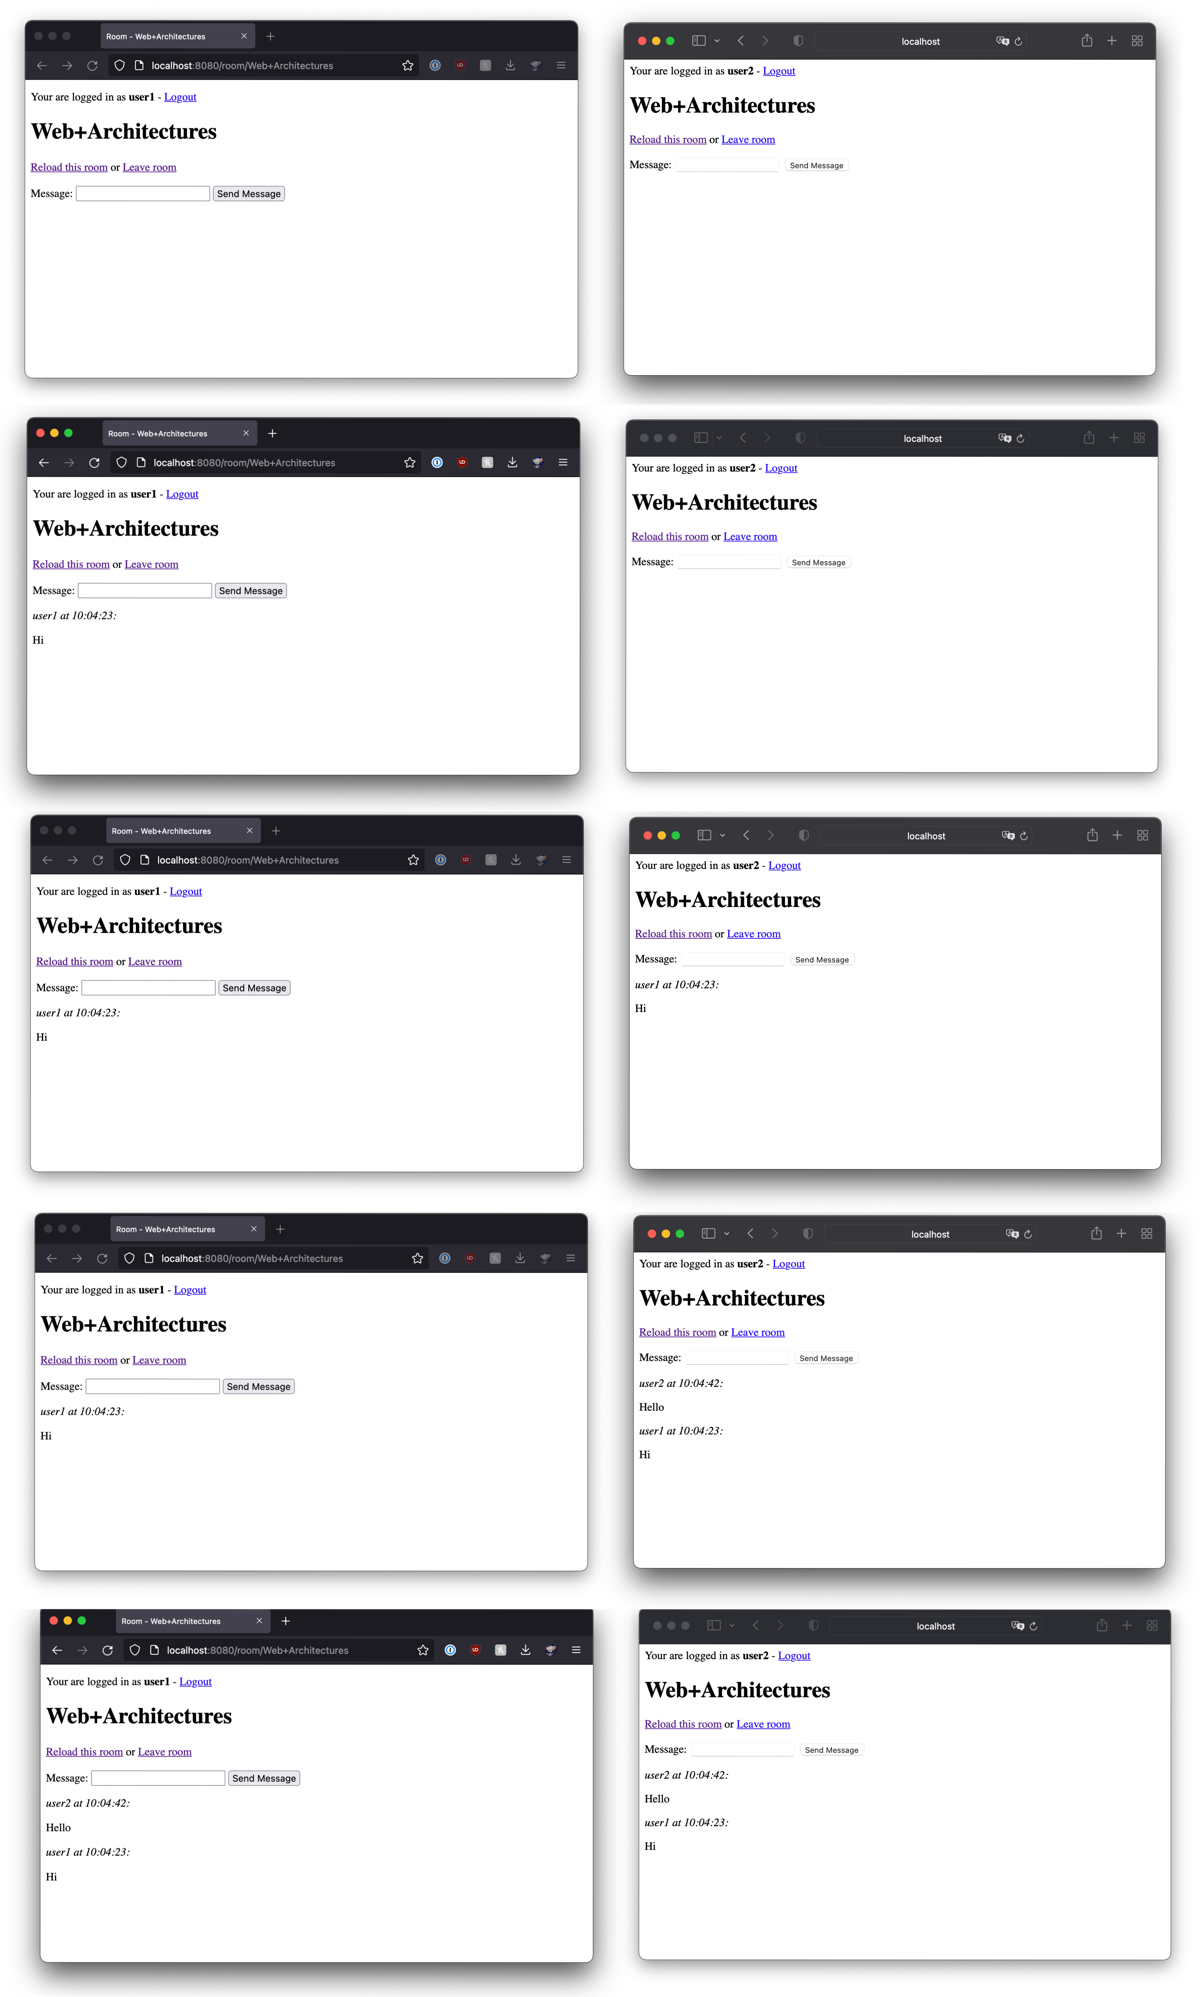
\includegraphics[scale=0.3]{images/03_impl/room/chat_all_steps}
\caption{Creation-process of \textit{user3}}
\label{fig:03_impl_servlets_admin_chat}
\end{figure}
% Explain figure
In a \textit{Room-Page}, multiple users can chat with each other, which is shown in \Fig{fig:03_impl_servlets_admin_chat}.
% The view
The \texttt{RoomServlet} owns a view called \texttt{Room.jsp}, which shows an HTML-Form, and lists all messages of the active Room.

% The active room
The active room is set as a Java Bean in the request. Therefore, the \texttt{JSP} view can access the model of the active room via \texttt{jsp:getProperty}. Then, all messages which belongs to the active room can be received via the \texttt{getMessages()} method of a \texttt{Room} model and can be listed in a \texttt{ul} element using a \texttt{for} loop. \Lst{lst:03_impl_servlets_room_bean} shows the implementation, how messages are listed in the room view.
% The listing
\begin{lstlisting}[label=lst:03_impl_servlets_room_bean, caption=List messages for a specific room, language=html]
<%@ page import="java.util.List" %>
<%@ page import="it.unitn.disi.webarch.chat.models.room.Message" %>
<jsp:useBean id="activeRoom" class="it.unitn.disi.webarch.chat.models.room.Room" scope="request" />
...
<body>
<%
List<Message> messages = activeRoom.getMessages();
for(Message message: messages) {
%>
  <div>
    <p><em><%= message.getUser() %> at <%= message.getFormattedDate() %>:</em></p>
    <p><%= message.getMessage() %></p>
  </div>
<% } %>
</body>
\end{lstlisting}

% Send messages
The HTML-form sends a \texttt{POST} request to itself. The request consists of an attribute called \texttt{message}, which is the message text of the user. After a \texttt{POST} request has been made, the \texttt{RoomServlet} constructs a new \texttt{Message} model, using the message text received from the \texttt{POST} request, and the username of the active user which is saved in the HTTP session. After that, the newly created \texttt{Message} model is added to the active \texttt{Room} model via the \texttt{addMessage} method. Finally, the page gets reloaded using the \texttt{doGet} method of the servlet. If the request is not valid (no room requested), the \texttt{RoomServlet} responses with a \texttt{400 - Bad Request} HTTP error. Otherwise, if the requested room does not exists, the \texttt{RoomServlet} responses a \texttt{404 - Not Found} HTTP error.

% Reload
To update newly created messages, the view reloads itself every 15 seconds using \texttt{<meta http-equiv="refresh" content="15">}.


\subsubsection{Admin}\label{subsubsec:03_impl_servlets_admin}
% Figure
\begin{figure}[h]
\centering
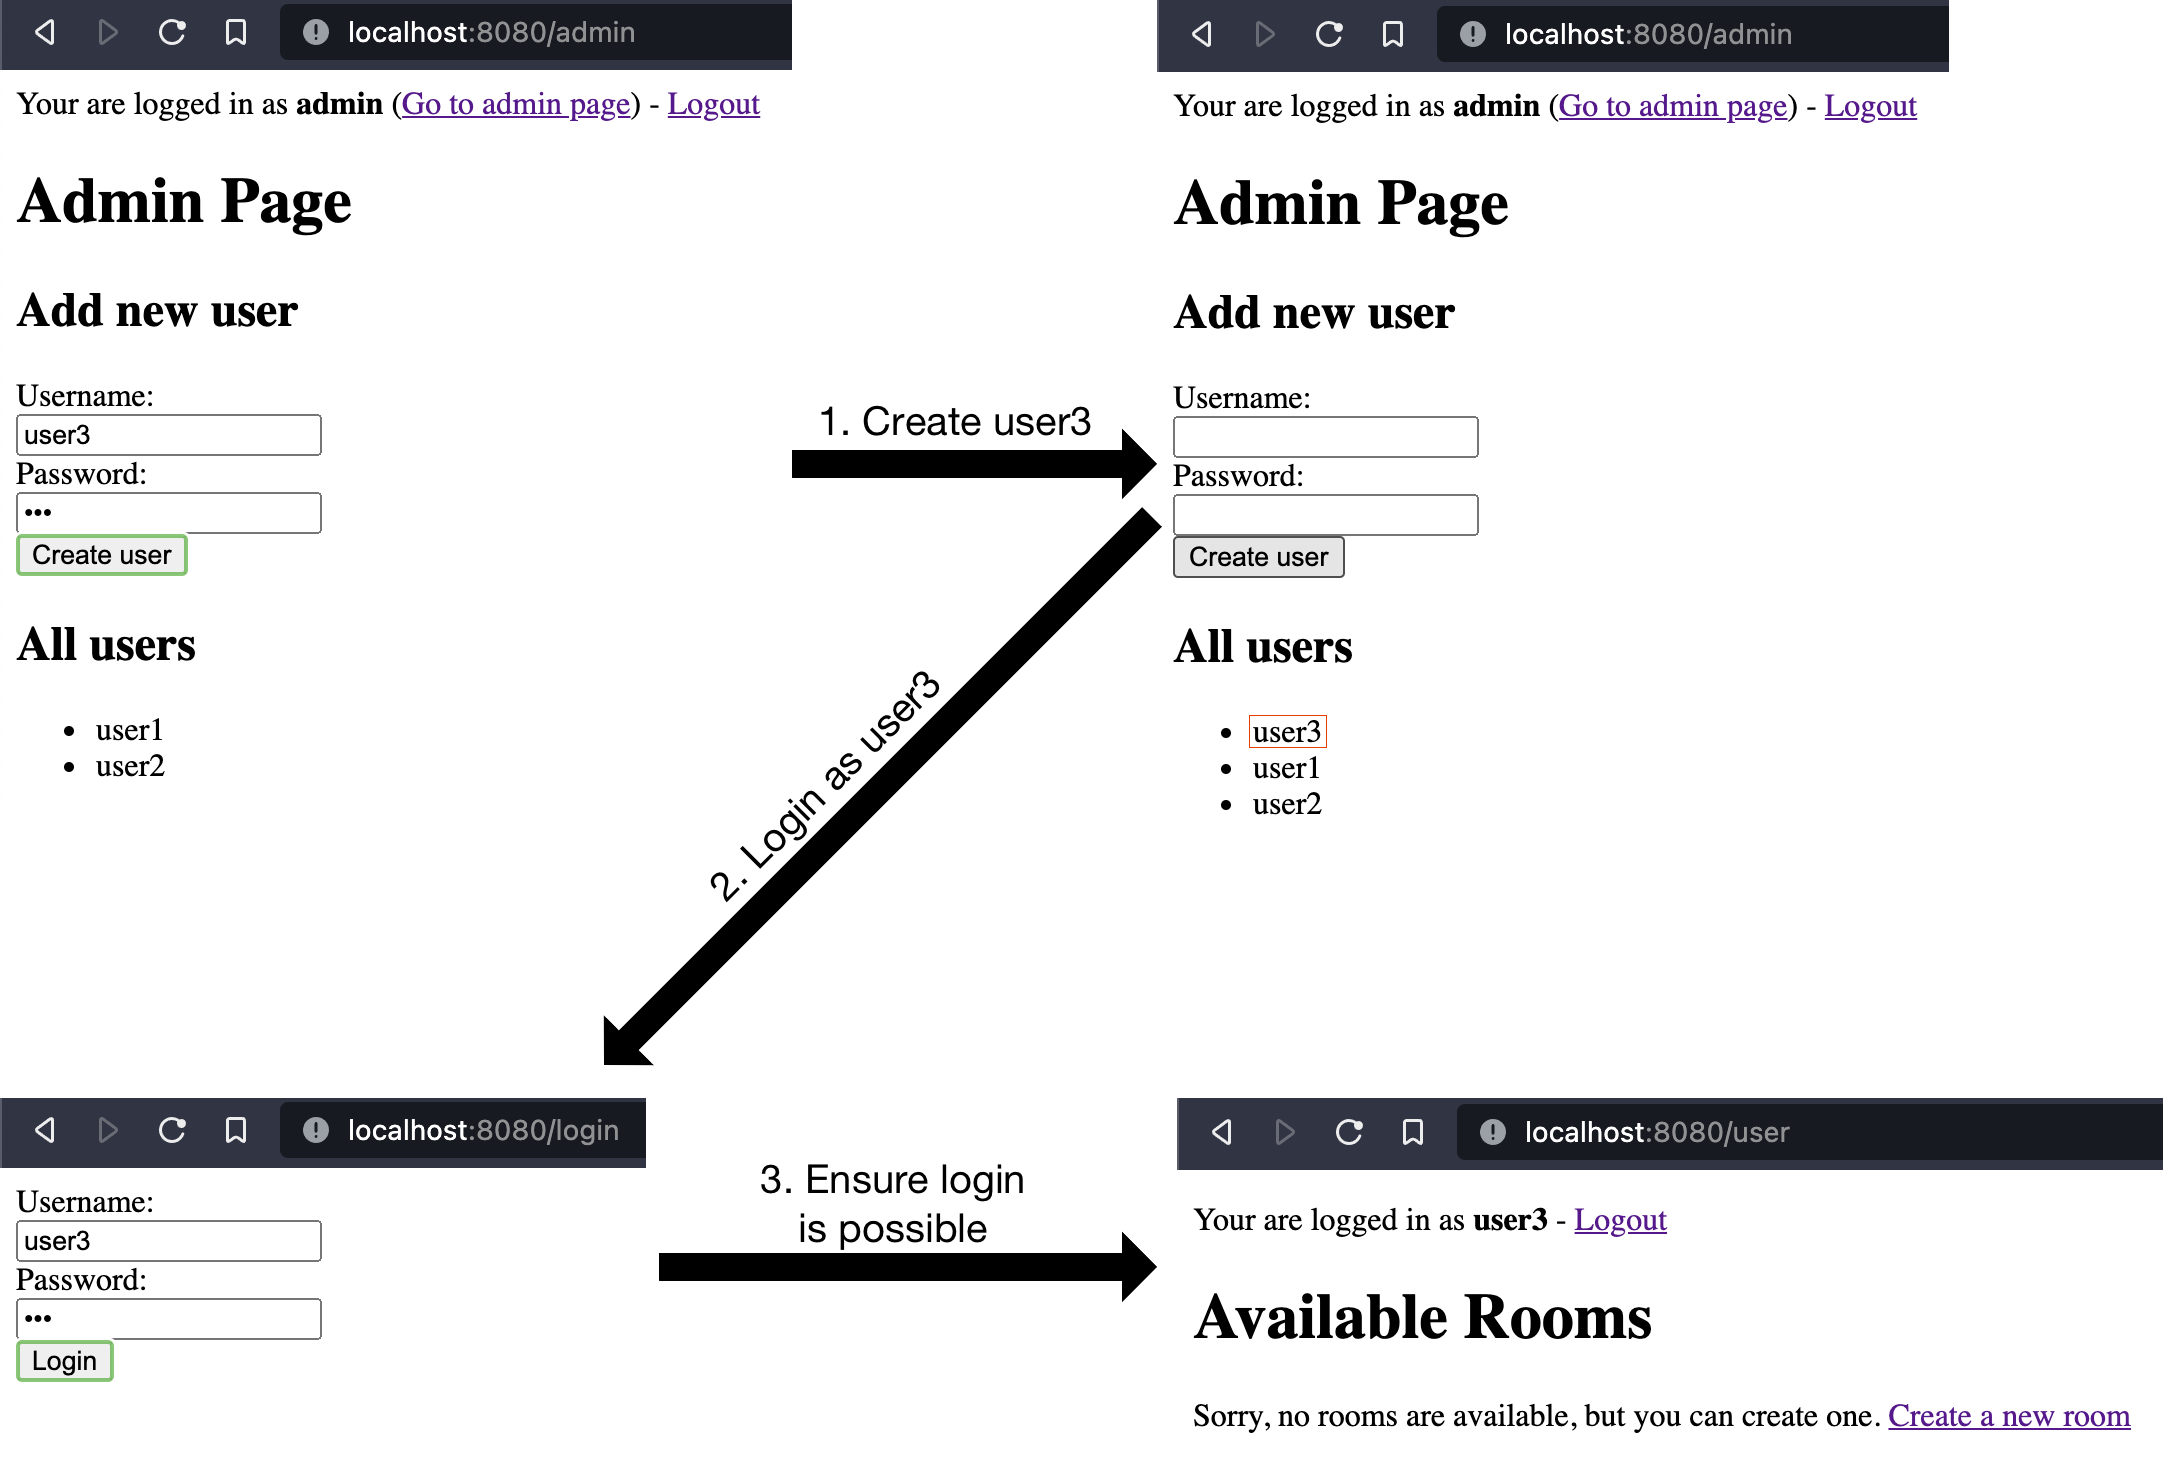
\includegraphics[scale=0.2]{images/03_impl/admin/create_user_all}
\caption{Creation-process of \textit{user3}}
\label{fig:03_impl_servlets_room_createall}
\end{figure}
% Explain figure
\Fig{fig:03_impl_servlets_room_createall} illustrates the successful creation-process of a user.
% HTML for
The admin can fill out the HTML-form of the \textit{Admin-Page}. After clicking submit, it will send the data (\texttt{username} and \texttt{password}) via a \texttt{POST} request to itself.
% Servlet
The \texttt{AdminServlet}, validates the the \texttt{POST} request attributes and checks if the user already exist If the user does not exist, the user will be add via the \texttt{addUser} method of the \texttt{UserStore}. As mentioned in SEC USERSTORE, the \texttt{UserStore} will write the user to the \texttt{users.txt} file.
% Check credentials
To check if the given credentials are valid, the \texttt{AdminServlet} checks if the given \texttt{username} and \texttt{password} are not \texttt{null}. Otherwise, the \texttt{AdminServlet} will response with a \texttt{400 - Bad Request} HTTP error. Additionally, the \texttt{AdminServlet} checks if the length of the \texttt{username} and \texttt{password} is bigger than 0, and if the \texttt{username} does not equal \textit{admin}. If one condition is not true, the \texttt{AdminServlet} executes the \texttt{doGet} method to reload itself.



% ==============
% ==============
\subsection{Filters}\label{subsec:03_impl_filters}

\subsubsection{Authentication}\label{subsubsec:03_impl_filters_auth}

\subsubsection{Admin}\label{subsubsec:03_impl_filters_admin}
